\section{Benutzeroberfl�che}

%\comment{Was sind die grundlegenden Anforderungen an die Benutzungsoberfl�che (Bildschirmlayout, Dialogstruktur, ...)?}


Im Folgenden wird die grobe Struktur des grafischen Benutzeroberfl�che dargestellt.
\\\\
Die Benutzeroberfl�che besteht aus einem einzelnen Fenster, das verschiedene Elemente enth�lt.
\begin{description}
\item[Dateimen�] Das Dateimen� bietet Men�punkte zum Anlegen eines neuen Automaten sowie zum Laden und Speichern einer Automatendefinition. Dar�ber hinaus kann das Programm mit einer Beenden-Men�punkt geschlossen werden
\item[Simulationsmen�] Das Simulationsmen� bietet einen Men�punkt um den aktuell angezeigten Automaten mit einem eingegebenen Eingabewort zu simulieren.
\item[Statusleiste] Die Statusleiste beinhaltet zus�tzliche Informationen zur Simulation und zum Ergebnis.
\end{description}
% hier Bilder von Nils
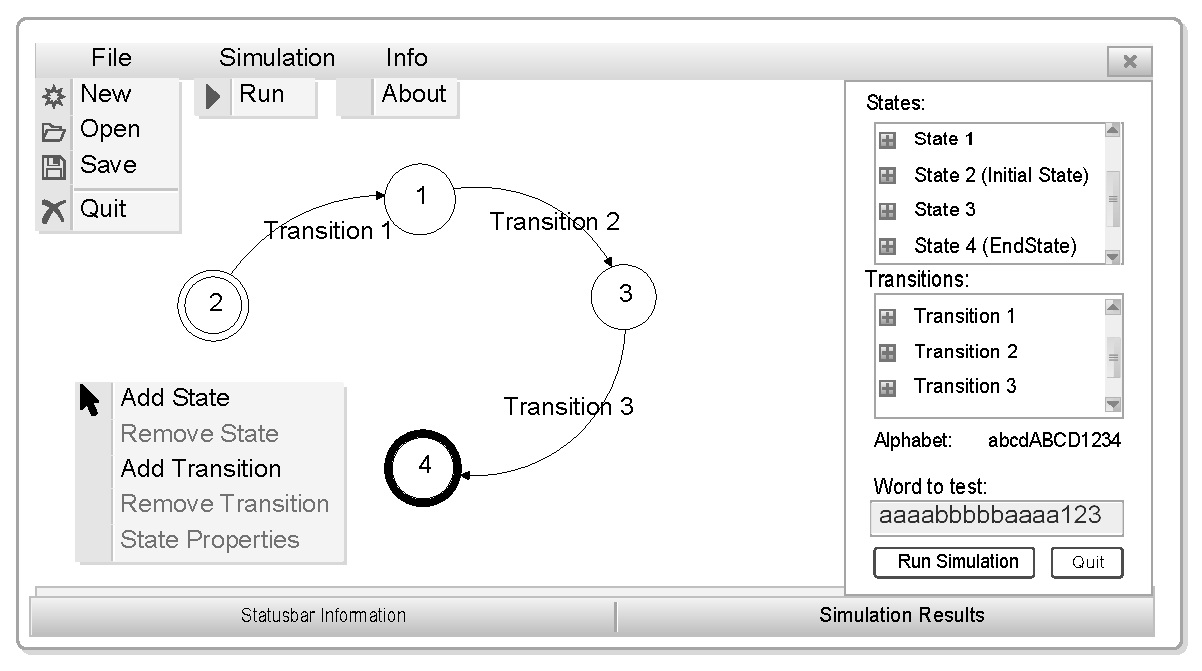
\includegraphics[width=\textwidth]{images/GUI_Mockup_final.eps}